\documentclass[authoryear,review,12pt]{elsarticle}
\usepackage{amssymb}
\usepackage{natbib}
\usepackage{multirow}
\usepackage{booktabs}
\usepackage{cha}
\usepackage{caption} % For caption customization
\captionsetup[figure]{labelformat=simple, labelsep=period, labelfont=sc}

\renewcommand\thefigure{S\arabic{figure}} 
\newcounter{myfig} % cre
\makeatletter
\renewcommand{\tablename}{Table S\@gobble}
\makeatotherounter{suppsection}
\renewcommand{\thesuppsection}{S\arabic{suppsection}}

\newcommand{\suppsection}[1]{
	\refstepcounter{suppsection}
	\section*{\thesuppsection. #1}\label{#1}
}

\usepackage{setspace}

\usepackage{lineno} % For line numbers
\usepackage{graphicx} % For including graphics

\usepackage{geometry}
\journal{Progress in Oceanography}	
\bibliographystyle{elsarticle-harv.bst}\biboptions{authoryear}
\usepackage[colorlinks = true, linkcolor=blue, urlcolor=blue, citecolor=blue]{hyperref}
\usepackage[nameinlink]{cleveref}
\crefname{figure}{Fig.}{Figs.}
\usepackage{titlesec}
\makeatletter
\def\ps@pprintTitle{%
}
\titleformat{\section}[hang]{\Large\bfseries}{S\thesection.}{1em}{}
\titleformat{\subsection}[hang]{\normalfont\bfseries}{S\thesubsection.}{1em}{}

\linespread{1.5}
\begin{document}
	\begin{frontmatter}
		\title{\textbf{\small Supplementary to} \\ Intraseasonal to interannual variability of zooplankton biomass and standing   stock inferred from ADCP backscatter in the eastern Arabian Sea}
		
		\address[inst1]{organization={CSIR-National Institute of Oceanography}, 
			addressline={Dona Paula},
			postcode={403004},
			state={Goa},
			country={India}}
		
		\address[inst2]{organization={Academy of Scientific and Innovative Research (AcSIR)}, 
			addressline={Ghaziabad},
			postcode={201002},
			state={Uttar Pradesh},
			country={India}}
		
		\address[inst3]{organization={CSIR-NIO, Regional Centre}, 
			addressline={Visakhapatnam},
			postcode={530017},
			state={Andhra Pradesh},
			country={India}}
		
		
		\author[inst1,inst2]{Ranjan Kumar Sahu}
		\author[inst1,inst2]{D. Shankar\corref{cor1}}
		\cortext[cor1]{Corresponding author}
		\ead{shankar@nio.res.in}
		\author[inst2,inst3]{P. Amol}
		\author[inst1,inst2]{S.G. Aparna}
		\author[inst1,inst2]{D.V. Desai}

	\end{frontmatter}
	\linenumbers
	The supplementary material consists of a detailed comparison with biomass climatology from \citep{aparna2022seasonal} (henceforth, A22). A brief introductory section about components of seasonal cycle and variabilities followed by overview of analysis tools used to identify the former are presented.
	
	\section{Comparison with biomass and ZSS climatology~of~A22}	
	\label{sec:comparison} 	
	It is observed that D215 is shallower at all locations and as a result a lower biomass and ZSS as seen in the climatology of the present study (\cref{fig:zsschlclimcomp}). The difference in D215 is prominent off Goa; while in the previous climatology  the D215 is deeper and lies along D23, in the present climatological data the D215 is shallower and lies $\sim$20--40 m above the D23 during January to April. A relatively lower biomass is present above z215 year round which reflects in overall lower ZSS of Goa and Mumbai. In the present data, the ZSS maximum off Mumbai occurs in March instead of February (A22), due to a lower ZSS value. The second maximum occurs in August and is less pronounced in recent data (\cref{fig:zsschlclimcomp} d1, d2). There is dramatic decrease in the minima off Mumbai that occurs in October and ZSS increases rapidly afterwards till February, and the minor peak seen in A22 is not observed off Mumbai. Off Kollam, higher biomass occurs from May to June in A22, and from May to June and September to November in the present study, with a ZSS minima in August. The higher ZSS on either side to this minima is less pronounced in A22. This difference in ZSS is clearly seen in the correlation, which is 0.60 off Kollam, while it is 0.94 and 0.98 off Mumbai and Goa, respectively. But the correlation reflects ZSS trend similarity, not magnitude deviation over time. In the present study, chl-a biomass peaks across all locations in August, and a minor peak off Mumbai. Off Kollam, revealing a zooplankton-phytoplankton relationship discrepancy consistent with A22 findings.

	\section{Seasonal cycle and analysis}
	\label{sec:seasonlity_analysis}
	The seasonal cycle constitutes of annual and semi-annual cycle, and the variability occurring in their respective period band. 
	\subsection{Interannual, annual, and intra-annual variability}
	\label{sec:seasonal_cycle}
	The biomass time series can be decomposed into distinct period bands spanning days to months. Among these diel vertical migration is the simplest variation, determining zooplankton biomass at a given depth with higher (lower) biomass at night (day), but it is not part of seasonal cycle and not the focus of our study. On a much longer time scale,  annual variability reflects changes over the course of a year often influenced by seasonal cycles like monsoons. For example, in the case of phytoplankton, upwelling favored by monsoonal winds can vary from year-to-year, thus determining the biomass for a given year uniquely. Interannual variability of first kind refers to variability occurring at periods beyond the annual scale (period $>~\sim$400 days), it's distinct from the second kind of interannual variability which is aperiodic and are deviations from seasonal cycle. Intra-annual variability arises due to the asymmetry of wind forcing between the summer and winter monsoons, and along with resonant forcing from equator leads to stronger semi-annual cycle (\citep{jensen2001arabian,schott20011}) specifically at SEAS similar to zooplankton biomass (Section 3.3). Hence, intra-annual variability captures fluctuations that occur between seasons, e.g., while both summer and winter monsoons are the growing season for chl-a at NEAS and SEAS, the strength of bloom varies with season. At a further lower temporal scale, the intraseasonal variability arises due to short-term (few days to 90 days) changes and dominates the zooplankton biomass and currents as discussed in Section 5.
	
	\subsection{Wavelet analysis and Lanczos filter}
	\label{sec:wavelet_lanczos}
	Before we understand wavelet analysis, it is imperative to have knowledge about Fourier analysis which decomposes a time series into sum of cosine and sine functions. The power spectrum of Fourier analysis shows peaks corresponding to period or frequency of a cycle and is meaningful for a cycle with known periodicity, e.g., annual and semi-annual cycle with known periodicity of 365 and 180 days, respectively. However, this technique can obscure the non stationary signals within the seasonal cycle variations of a time series \citep{amol2014observed,chaudhuri2020observed}. In a real world scenario of oceanography, no cycle is continuous when we consider it's strength and extent of cycle. Wavelet analysis was developed to counter this drawback as it provides a representation of time series in time-frequency domain \citep{torrence1998practical}. It employs wavelets, a localized wave-like functions that can be customized by varying wavelet's scale and position along the time series to identify periodic/stationary and irregular non-stationary patterns and their strength with time. This analysis is routinely used in time series data in the field of oceanography and geophysics, biomedical engineering and signal processing etc.
	
	Wavelet analysis has a crucial role to identify the seasonal cycle of zooplankton biomass and ZSS, and understanding of the method to interpret the wavelet figure is vital. Biomass time series at 40 and 104 m is chosen and decomposed to time (abscissa) vs frequency (ordinate) domain. While the time is linearly progressing, the inverse of frequency is represented as period for ease of understanding in logarithm scale (Fig. 6). The horizontal lines from the ordinate represents a specific period, and the color of wavelet spectra along the line shows intensity and continuity of cycle corresponding to that period. There is two more things keep in mind, 1) The cone of influence (CoI), beyond which edge effects (because of finite data) distort the spectrum; 2) Contours of statistical significance, showing patterns and features that are unlikely to have occurred by chance \citep{torrence1998practical}. For a cyclic feature to be labeled as present in time series, it must be within the CoI and be statistically significant. Say, in (Fig. 6), at the annual scale (365-days period) off Mumbai, intensity of wavelet spectra is high, it lies well within CoI, and is statistically significant. The semi-annual cycle along with bursts in intraseasonal scale is also seen. However, cross period comparison can't be made beyond a certain period due to emphasis of normalization on wavelet power at higher period \citep{maraun2004cross}. And for this need of comparison we move to filtering techniques.
	
	The Lanczos filter used is a digital construct that allows/restricts signals within period
	of interest \citep{duchon1979lanczos}. It is digital analogous to physical filters used in biology labs to filter zooplankton within a size range. While the wavelet analysis gives idea about variation of biomass occurring with time at all period, the Lanczos filtered data shows variation of biomass within a period band of interest. Hence, the range, distribution and intensity of biomass in a period band could be compared with another band unlike wavelet analysis where comparison can be made in one point of time to another at same or nearby period only. Note that the negative (positive) numbers in filtered biomass is representing deviation i.e., decrease (increase) from the mean in that distinct band. In the present context, we have made comparison between multiple bands as discussed in section 3.3 onward. Taking the time series at a single depth of 40~m in all three bands shows that the intraseasonal variability is dominating and its magnitude increases as we move towards equator Fig. 11.
	
\newpage
\linespread{1}	
\footnotesize 	
\bibliography{bs_citations_mod} % Specify your .bib file
\bibliographystyle{elsarticle-harv.bst}





\newpage
\newgeometry{top=1in, bottom=1in} 	

\begin{table}[t]
	
	{\footnotesize
		\captionsetup{justification=justified,font=footnotesize,skip=0.05\baselineskip,width*=\columnwidth} % Adjust the spacing above and below the caption
		\caption{\newline The mean, standard deviation at 40 and 104 m of zooplankton biomass (mg~m$^{-3}$), and in each of the distinct variability band, and standard deviation of ZSS (gm~m$^{-2}$, 24--140 m integrated biomass)  and chl-a (mg~m$^{-3}$) at 7 mooring sites are tabulated. The standard deviation of Chl and ZSS is based on the monthly climatological data while the rest are based on the respective daily data.}
		
		\begin{adjustwidth}{-0.8in}{0in} 
\begin{tabular}{ccccccllccc}
	\multicolumn{1}{c|}{\multirow{2}{*}{\begin{tabular}[c]{@{}c@{}}Mooring\\  location\end{tabular}}} & \multicolumn{2}{c|}{40 m biomass}                      & \multicolumn{2}{c|}{104 m biomass}                  & \multicolumn{1}{c|}{\multirow{2}{*}{\begin{tabular}[c]{@{}c@{}}decrease \\ with depth \\ (40m – 104m)\end{tabular}}} & \multicolumn{2}{c|}{\begin{tabular}[c]{@{}c@{}}standard \\ deviation\end{tabular}} & \multicolumn{3}{c}{\begin{tabular}[c]{@{}c@{}}standard deviation \\ at 40 m biomass\\ in distinct bands\end{tabular}} \\ \cline{2-5} \cline{7-11} 
	\multicolumn{1}{c|}{}                                                                             & \multicolumn{1}{c|}{Mean} & \multicolumn{1}{c|}{SD}    & \multicolumn{1}{c|}{Mean} & \multicolumn{1}{c|}{SD} & \multicolumn{1}{c|}{}                                                                                                & \multicolumn{1}{c|}{Chl}                 & \multicolumn{1}{c|}{ZSS}                & \multicolumn{1}{c|}{intraseasonal}              & \multicolumn{1}{c|}{intra-annual}              & annual             \\ \hline
	Okha                                                                                              & 230.42                    & 22.84                      & 151.68                    & 25.58                   & 78.74                                                                                                                & 0.25                                     & 1.55                                    & 10.71                                           & 10.63                                          & 3.73               \\
	Mumbai                                                                                            & 272.86                    & \multicolumn{1}{c|}{34.95} & 182.24                    & 30.34                   & 90.62                                                                                                                & 0.13                                     & 2.42                                    & 11.79                                           & 13.92                                          & 6.93               \\
	Jaigarh                                                                                           & 278.45                    & 36.52                      & 182.96                    & 48.89                   & 95.49                                                                                                                & 0.05                                     & 2.34                                    & 15.05                                           & 14.51                                          & 9.05               \\
	Goa                                                                                               & 235.22                    & 30.34                      & 163.02                    & 36.54                   & 72.2                                                                                                                 & 0.15                                     & 1.73                                    & 12.73                                           & 13.96                                          & 6.43               \\
	Udupi                                                                                             & 247.81                    & 34.37                      & 169.37                    & 38.8                    & 78.43                                                                                                                & 0.55                                     & 1.74                                    & 12.87                                           & 16.81                                          & 6.94               \\
	Kollam                                                                                            & 272.56                    & 54.94                      & 198.89                    & 50.08                   & 73.67                                                                                                                & 0.68                                     & 1.13                                    & 14.99                                           & 15.99                                          & 6.97               \\
	KanyaKumari                                                                                       & 207.07                    & 30.42                      & 167.63                    & 20.89                   & 39.44                                                                                                                & 0.51                                     & 0.46                                    & 11.98                                           & 8.77                                           & 3.64              
\end{tabular}
	\end{adjustwidth}
	}
	\label{mytable:b}
\end{table}

\begin{figure}[htbp]
	\centering
	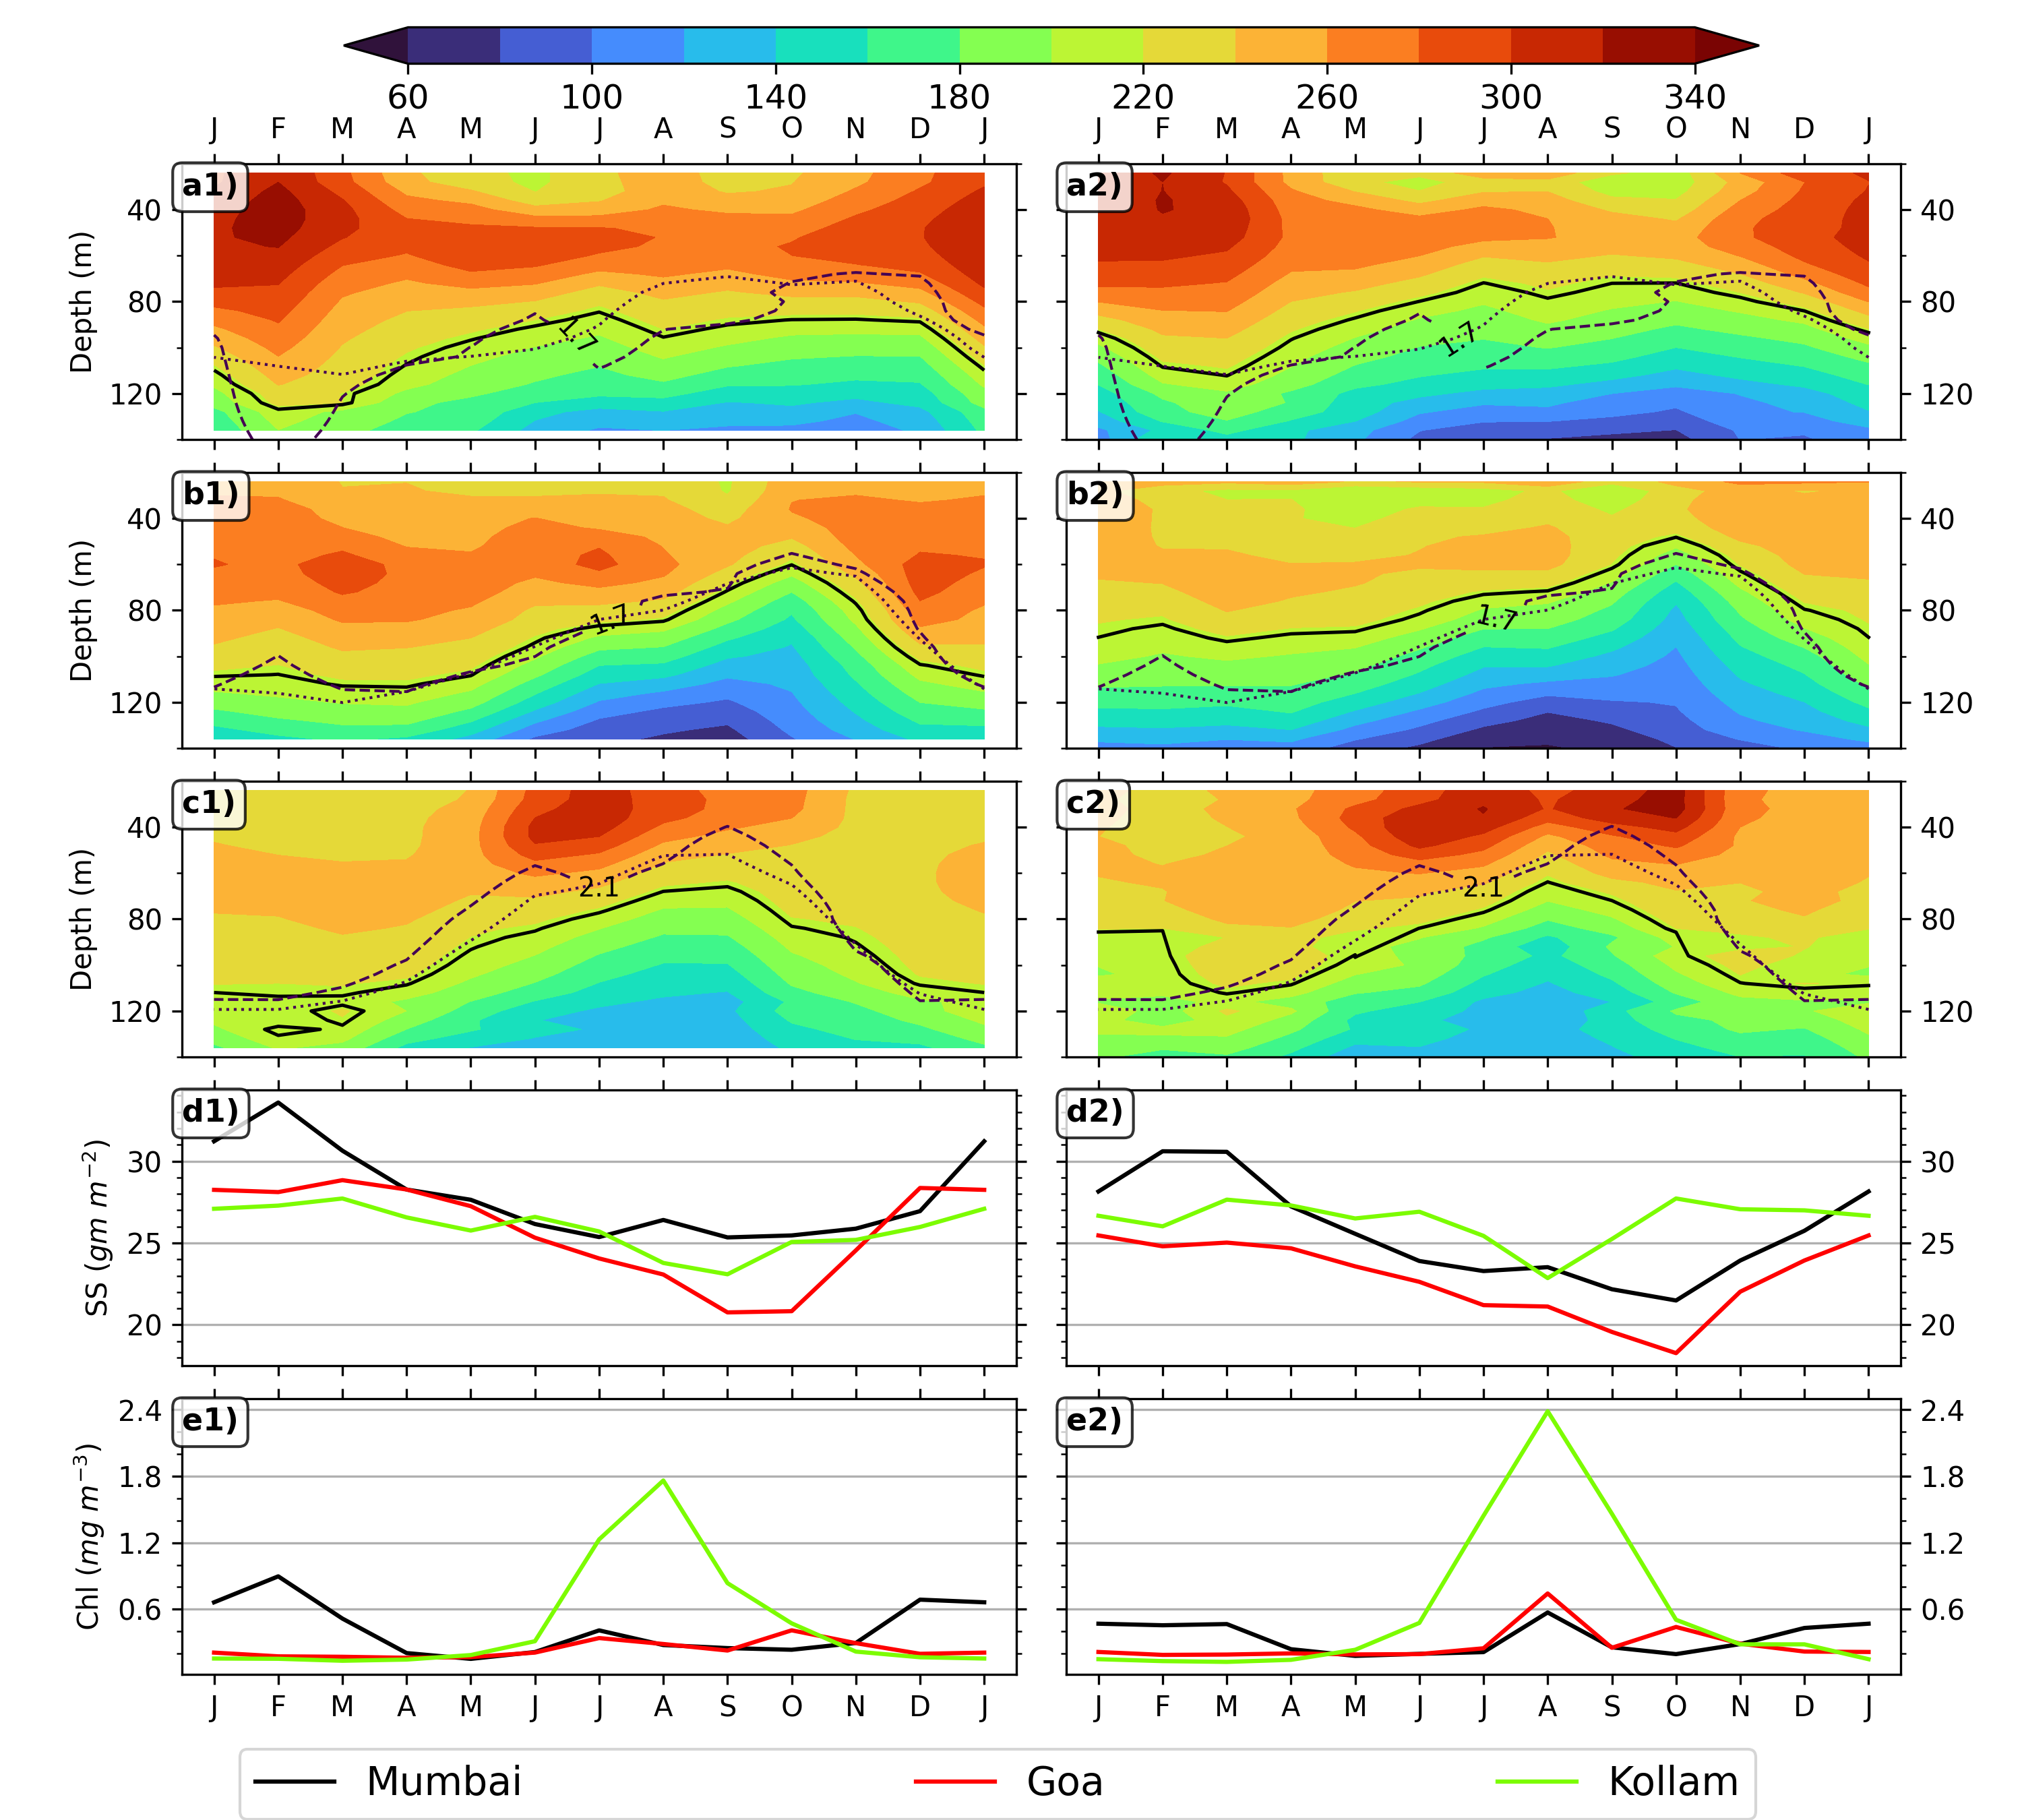
\includegraphics[width=\textwidth]{./figures/aparna_ranjan_climatology_comparison.png} 
	\captionsetup{justification=justified,font=footnotesize,skip=0.05\baselineskip,width=\textwidth}
	\caption{Monthly climatology of zooplankton biomass is shown in left panels for 3 locations which were earlier used in \citep{aparna2022seasonal}; a1, b1 \& c1 is the biomass climatology for Mumbai, Goa and Kollam, d1 is for ZSS climatology (24--140 biomass integral), e1 is for chl-a biomass climatology; a2, b2, c2, d2 \& e2 is same but based on data from 2017 to 2023. The D215 is shown in solid black. The dashed line represents the depth of 23 $^\circ$C isotherm; oxygen contours are shown in dotted lines and labeled for each location.}
	\label{fig:zsschlclimcomp}
	\refstepcounter{myfig}\label{myfig:a}
\end{figure}

\begin{figure}[htbp]
	\centering
	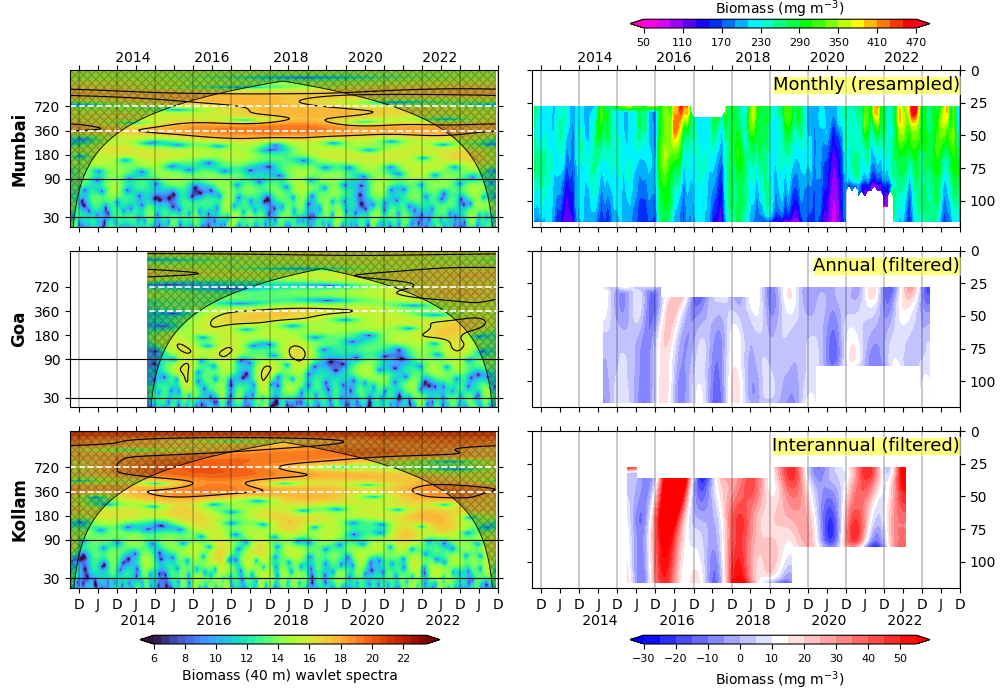
\includegraphics[width=\textwidth]{./figures/6kollam_annual_interannual_and_wavelet.png} 
	\captionsetup{justification=justified,font=footnotesize,skip=0.05\baselineskip,width=\textwidth}
	\caption{The wavelet spectra off Mumbai, Goa, and Kollam from 2012 to 2023 is shown in the left panel. While NEAS shows strong annual cycle, it is weaker off CEAS. Further south, the cycles corresponding to 720 days ($\sim$2 year) shows up prominently in spectra. The right panel shows monthly resampled biomass off Kollam, and it's annual and interannual filtered components, and the later two share same color scale.}
	\label{fig:interannual_variability}
	\refstepcounter{myfig}\label{myfig:b}
\end{figure}

\begin{figure}[htbp]
	\centering
	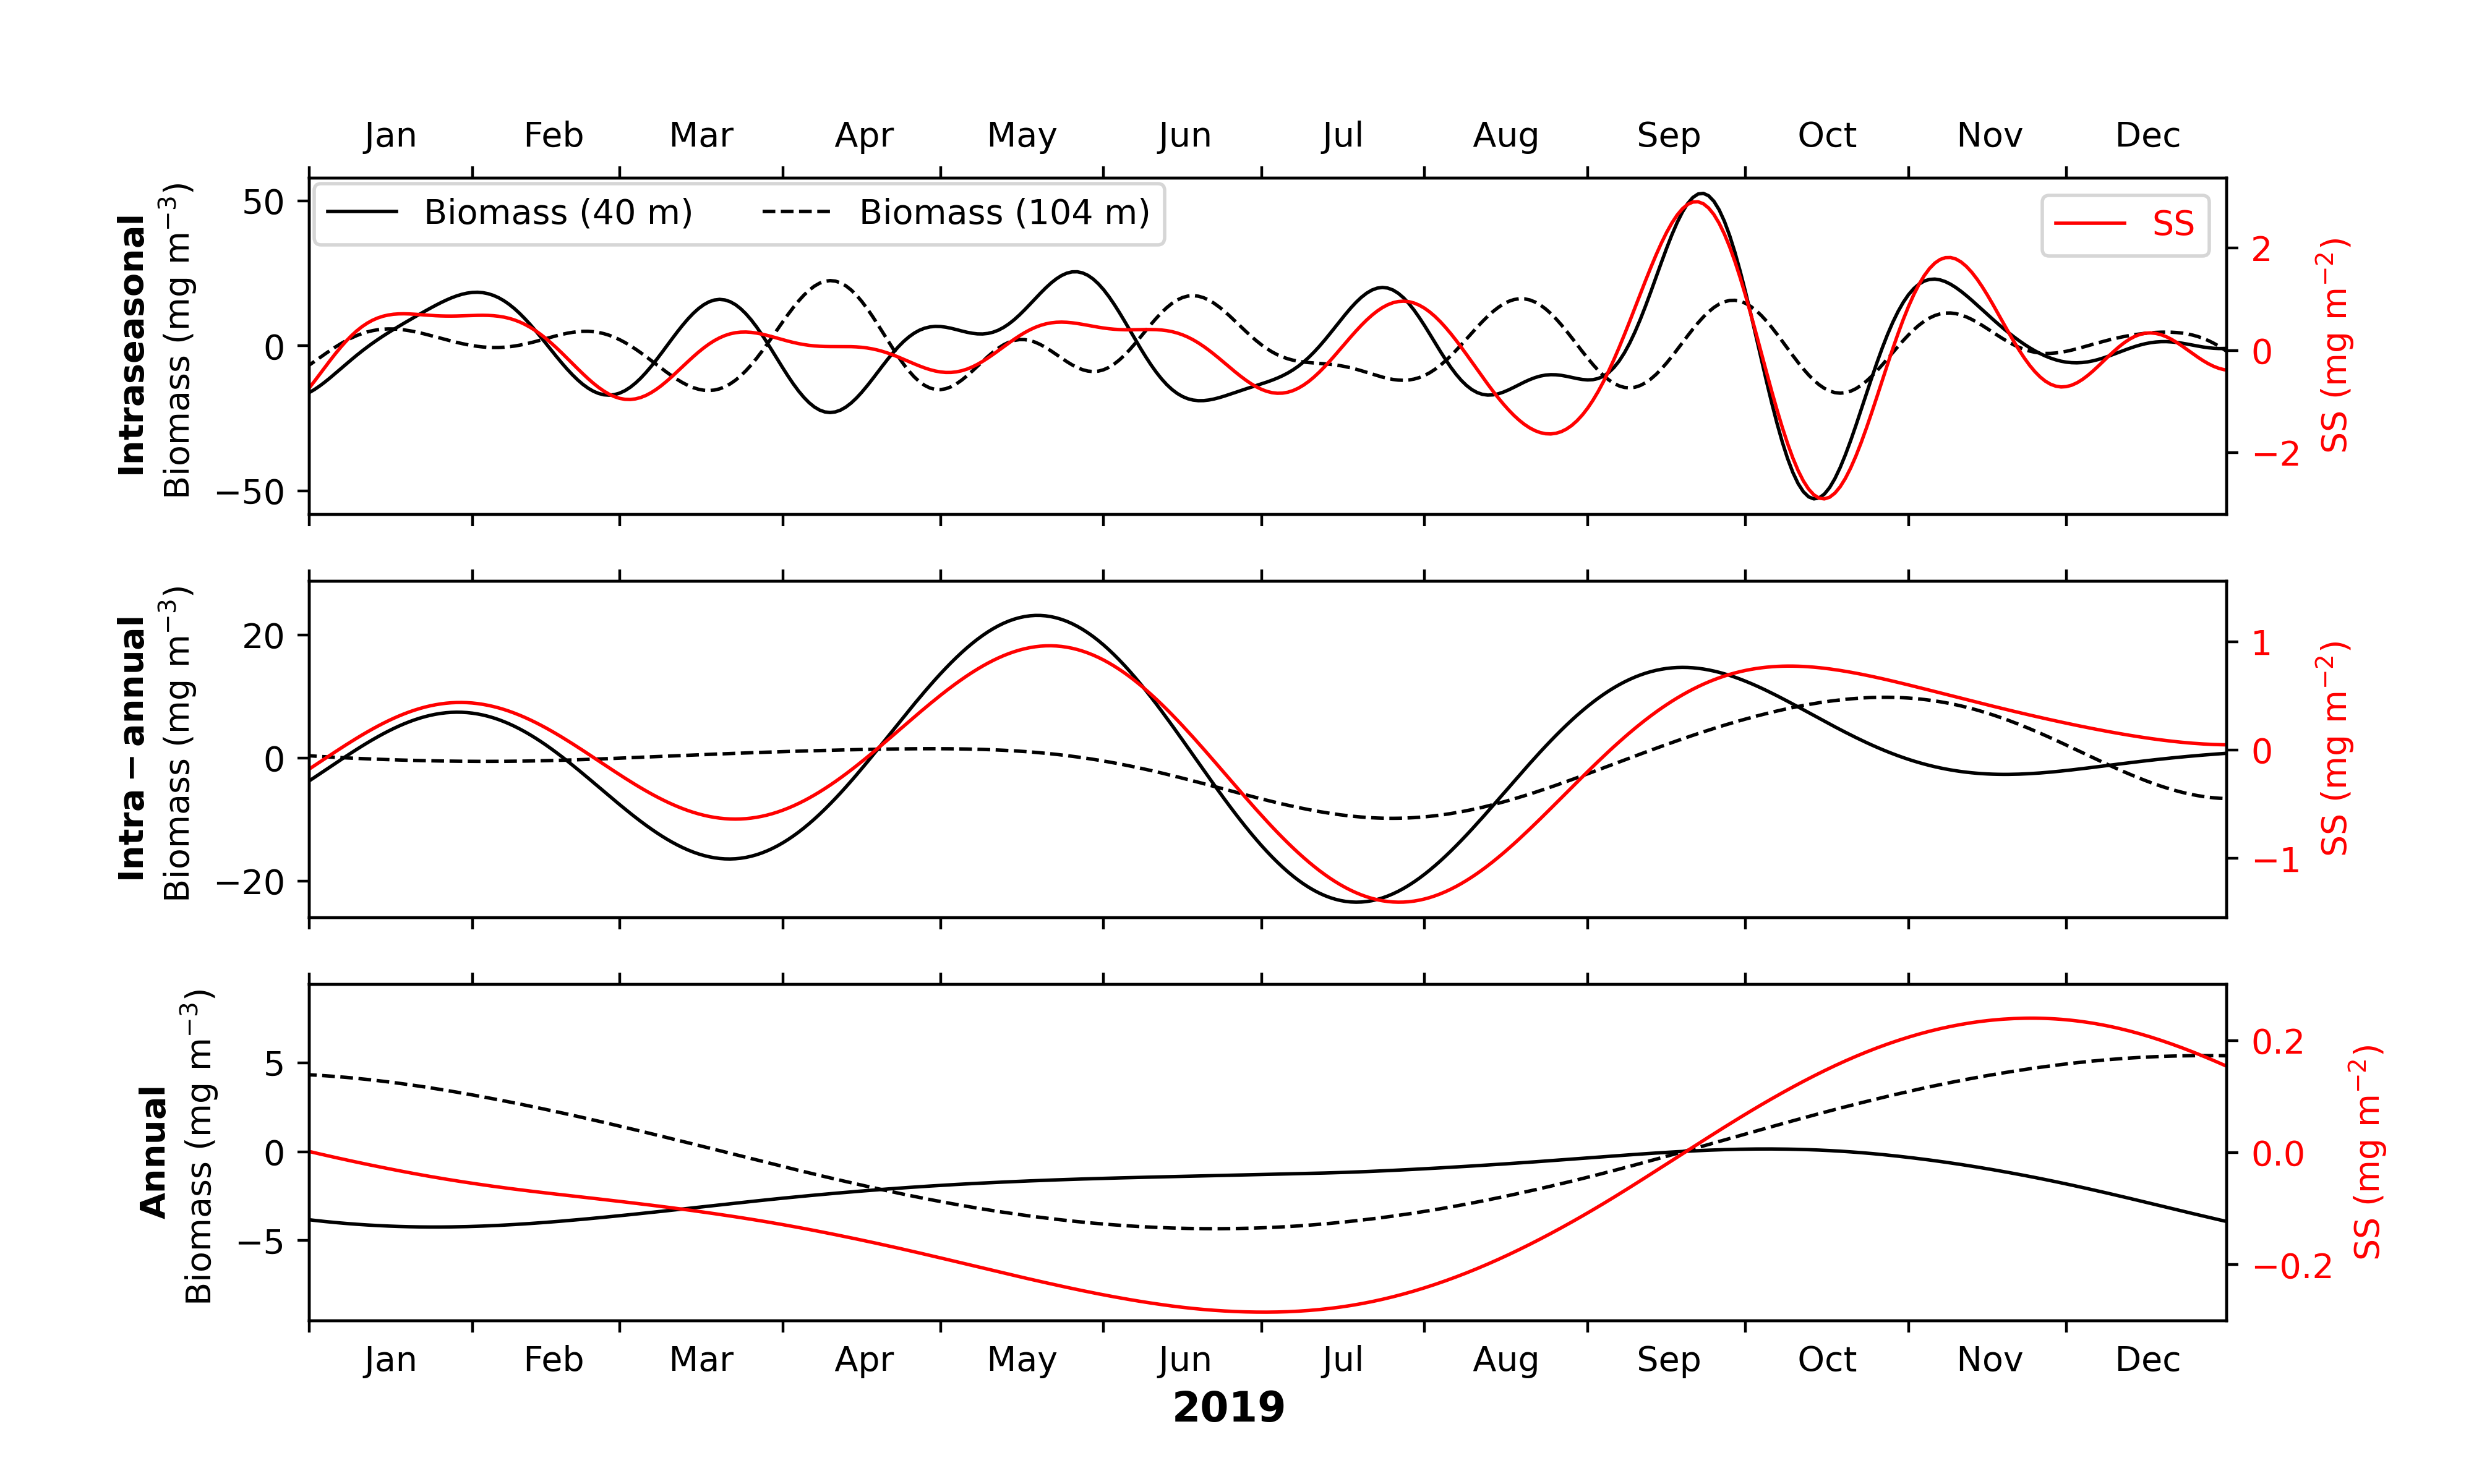
\includegraphics[width=\textwidth]{./figures/ss_biomass_comparison_intraseasonal_band.png} 
	\captionsetup{justification=justified,font=footnotesize,skip=0.05\baselineskip,width=\textwidth}
	\caption{The 40 and 104 m biomass in comparison with ZSS (column integrated standing stock). The biomass at 104 m may or may not be in phase with upper ocean biomass at 40 m, thereby enhancing or diminishing ZSS variation and it is seen at all the distinct bands of variability.}
	\label{fig:40_104_biomass_zss}
	\refstepcounter{myfig}\label{myfig:c}
\end{figure}


\begin{figure}[htbp]
	\centering
	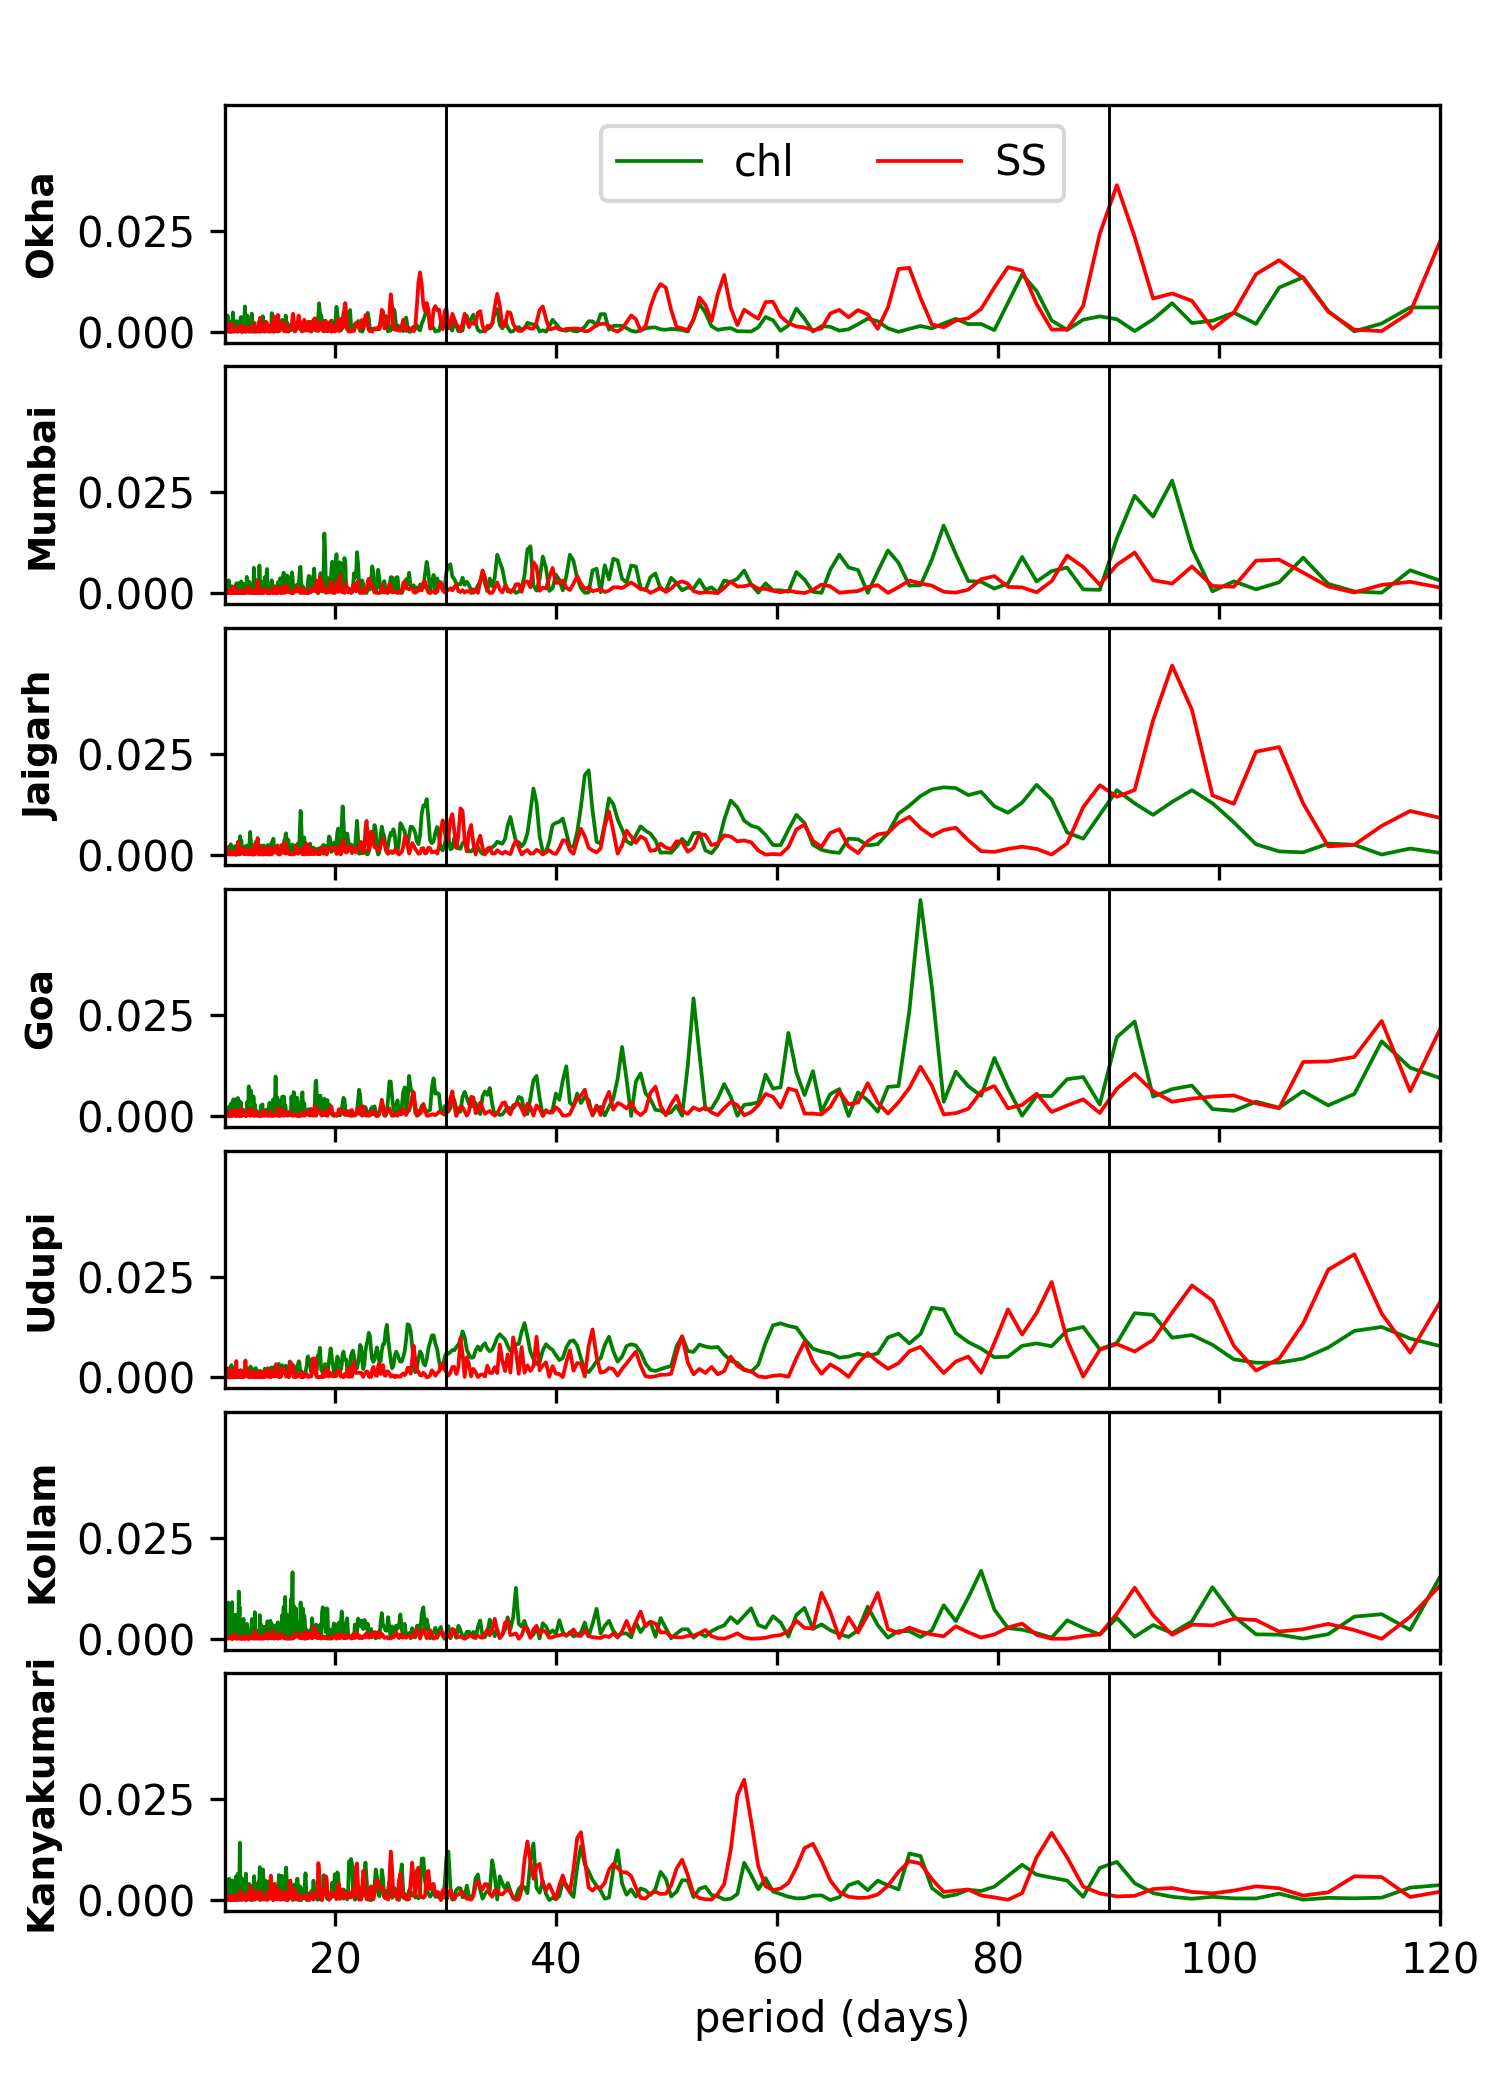
\includegraphics[width=0.9\textwidth]{./figures/Lombscargle_periodogram_daily_chl_ss.png} 
	\captionsetup{justification=justified,font=footnotesize,skip=0.05\baselineskip,width=\textwidth}
	\caption{Lomb-Scargle periodogram of daily ZSS and chl at the mooring sites. Vertical lines mark the 30 and 90 days period. The periodogram shows presence of variability in ZSS and Chl, at the high and low-frequency component of intraseasonal variability.}
	\label{fig:zss_chl_lombscarge}
	\refstepcounter{myfig}\label{myfig:e}
\end{figure}

\end{document}